\documentclass[11pt,a4paper,oneside]{scrartcl}

\usepackage[utf8]{inputenc}
\usepackage[ngerman]{babel}
\usepackage{amsmath, amssymb, amsthm} 
\usepackage{graphicx, tikz} 
\usepackage{hyperref} 
\usepackage{tabularx}
\usepackage[linesnumbered,ruled,vlined]{algorithm2e}

\newtheorem{satz}{Satz}[section]
\newtheorem{lemma}[satz]{Lemma}
\newtheorem{proposition}[satz]{Proposition}
\newtheorem{definition}[satz]{Definition}
\newtheorem{bemerkung}[satz]{Bemerkung}
\usepackage{tikz}
\usetikzlibrary{shapes.geometric, arrows}

\tikzstyle{startstop} = [rectangle, rounded corners, minimum width=3cm, minimum height=1cm,text centered, draw=black, fill=red!30]
\tikzstyle{prozess} = [rectangle, minimum width=3cm, minimum height=1cm, text centered, draw=black, fill=orange!30]
\tikzstyle{arrow} = [thick,->,>=stealth]

\begin{document}

\title{Ausarbeitung zum Thema AdaBoost}
\subtitle{Bachelor-Seminar "`Top 10 Algorithms in Data Mining"'}

\author{Marius Graf}
\date{\today}

\maketitle

\tableofcontents

\begin{abstract}
    \noindent\textbf{Abstract:}
    Diese Arbeit beschäftigt sich mit dem AdaBoost-Algorithmus, einer Ensemble-Methode im maschinellen
    Lernen, die mehrere schwache Lerner kombiniert, um ein präzises Gesamtmodell zu erstellen. Die Arbeit
    erklärt die Grundlagen des Boosting-Konzepts, den Ablauf des AdaBoost-Algorithmus und umreißt seine Anwendung in
    der Praxis. Zuletzt werden auch die Vor- und Nachteile von AdaBoost diskutiert sowie einige Erweiterungen und Variationen
    des Algorithmus für unterschiedliche Problemstellungen dargestellt.
\end{abstract}
\newpage

\section{Einleitung}
Data Mining analysiert große Datenmengen, um Muster und Zusammenhänge zu erkennen,
wobei Methoden aus Statistik, Machine Learning und Datenbanktechnologie eingesetzt werden.
Es spielt eine zentrale Rolle in Forschung und Industrie, um Erkenntnisse zu gewinnen und
Entscheidungen zu unterstützen. AdaBoost gehört zu den
\emph{Ensemble-Methoden}, die mehrere Modelle kombinieren, um präzisere Vorhersagen zu treffen.
Diese Arbeit konzentriert sich auf AdaBoost, der Beobachtungen gewichtet, um zuvor falsch bzw. schlecht vorhergesagte
Datenpunkte besser vorherzusagen.
\section{Grundlagen des Boosting}
Boosting ist eine Ensemble-Technik im Machine Learning, die mehrere sog. \emph{\glqq schwache Lerner\grqq} kombiniert,
um ein präzises Gesamtmodell zu erstellen. Als \emph{schwacher Lerner} wird ein Modell bezeichnet, das nur einen geringen
Zusammenhang in den Daten lernen kann und dessen Vorhersagen daher nur etwas besser als zufälliges Raten sind.
In jeder Iteration wird ein solches Modell trainiert, das falsche
Vorhersagen der vorherigen Modelle korrigiert, indem es die Gewichtung der Trainingsdaten anpasst.
Das Ziel ist es, den systematischen Fehler (\emph{Bias}) des Modells zu reduzieren und die Genauigkeit
schrittweise zu verbessern, indem es sich auf schwierig zu klassifizierende Datenpunkte konzentriert.

\begin{figure}[h]
    \centering
    \includegraphics[width=0.8\textwidth]{"./figures/Boosting_Graph"}
    \caption{Flussdiagramm zur Veranschaulichung des Boosting-Konzepts}
\end{figure}

\subsection*{Beispiel:}
Stellen wir uns vor, wir möchten ein Modell entwickeln, das den Preis von
Häusern basierend auf verschiedenen Merkmalen wie Größe, Lage, Anzahl der
Zimmer und Baujahr vorhersagt.

\begin{table}[h]
    \centering
    \begin{tabularx}{\textwidth}{|X|X|X|X|}
    \hline
    \textbf{Haus} & \textbf{Größe $[m^2]$} & \textbf{Lage} & \textbf{Preis} \\
    \hline
    Haus 1        & 100                    & Zentrum       & 500.000€       \\
    \hline
    Haus 2        & 150                    & Vorort        & 300.000€       \\
    \hline
    Haus 3        & 80                     & Zentrum       & 400.000€       \\
    \hline
    Haus 4        & 120                    & Ländlich      & 200.000€       \\
    \hline
\end{tabularx}
    \caption{Beispielhafte Daten für Hauspreise basierend auf Größe und Lage}
\end{table}

\begin{itemize}
    \item Wir entscheiden uns zunächst für ein sehr einfaches Modell (schwacher Lerner),
          das den Preis nur anhand der Größe des Hauses vorhersagt.
          Dieses Modell geht davon aus, dass alle anderen Merkmale keinen
          Einfluss auf den Preis haben.
    \item In Wirklichkeit variieren die Hauspreise jedoch nicht nur aufgrund
          ihrer Größe, sondern auch aufgrund anderer Faktoren. Ein kleines Haus in einer
          begehrten Lage könnte teurer sein als ein großes Haus in einer weniger beliebten
    \item Da unser Modell nur die Größe berücksichtigt und alle anderen Faktoren ignoriert,
          wird es systematisch den Preis von Häusern in begehrten Lagen unterschätzen und den Preis
          von Häusern in weniger beliebten Gegenden überschätzen. Dieser systematische Fehler in den
          Vorhersagen ist der \textbf{Bias}.
\end{itemize}

In mehreren Iterationen wird beim Boosting nun das Gewicht der Datenpunkte so angepasst, dass sich das
zweite Modell auf genau die Datenpunke fokussiert, welche zuvor falsch bzw. besonders schlecht vorhergesagt wurden.
Somit ist hier eine deutlich größere Anpassung der Vorhersage zu erkennen als bei den Datenpunkten, die zuvor
relativ gut vorhergasagt wurden.

\begin{table}
    \centering
    \begin{tabularx}{\textwidth}{|X|X|X|X|X|X|}
    \hline
    \textbf{Haus} & \textbf{Größe $[m^2]$} & \textbf{Lage} & \textbf{Preis} & \textbf{Vorhersage (It. 1)} & \textbf{Vorhersage (It. 2)} \\
    \hline
    Haus 1        & 100                    & Zentrum       & 500.000€       & 450.000€                    & 490.000€                    \\
    \hline
    Haus 2        & 150                    & Vorort        & 300.000€       & 350.000€                    & 310.000€                    \\
    \hline
    Haus 3        & 80                     & Zentrum       & 400.000€       & 380.000€                    & 405.000€                    \\
    \hline
    Haus 4        & 120                    & Ländlich      & 200.000€       & 250.000€                    & 210.000€                    \\
    \hline
\end{tabularx}
    \caption{Beispielhafte Daten für Hauspreise und wie Boosting den Bias in mehreren Iterationen reduziert}
\end{table}
Zuletzt werden alle schwachen Lerner zu einem \emph{starken Lerner} als Ensemble zusammengefügt, wobei die Vorhersagen
der einzelnen Modelle entsprechend ihrer individuellen Präzision gewichtet werden.
\section{Der AdaBoost Algorithmus}
\subsection*{Einführung}
AdaBoost, kurz für \glqq Adaptive Boosting\grqq, wurde in den 1990ern von Yoav Freund und Robert Schapire für die binäre
Klassifikation konzipiert und hat das Feld des maschinellen Lernens maßgeblich geprägt. Während Boosting-Methoden
allgemein iterativ arbeiten und Fehler der vorherigen Modelle korrigieren, zeichnet sich AdaBoost durch seine spezielle
Methode zur Gewichtungsanpassung der Datenpunkte aus. In jeder Trainingsiteration erhöht AdaBoost gezielt die Gewichtung
der falsch klassifizierten Datenpunkte, wodurch er kontinuierlich seine Vorhersagegenauigkeit verbessert. Dieser
einzigartige und adaptive Ansatz zur Fehlerkorrektur unterscheidet AdaBoost von anderen Boosting-Methoden und hat
nicht nur die Effizienz von Boosting-Methoden für binäre Klassifikationsprobleme unter Beweis gestellt, sondern auch zu
zahlreichen Weiterentwicklungen in diesem Bereich angeregt. \cite{WuKumar2009}

\subsection*{Notation}
\begin{itemize}
    \item Sei $\mathcal{X}$ die Menge der Features mit $\left|\mathcal{X}\right| = n$
          (Anzahl der Features) und $\mathcal{Y}$ die Menge der Labels, die gelernt werden sollen.
          Dabei ist $\mathcal{Y}=\{-1, +1\}$ bei binärer Klassifikation. Ein Trainingdatensatz $D$ besteht aus $m$ Einträgen,
          welche Features mit Labels verbinden:
          $$
              D=\{(\boldsymbol{x}_i, y_i)\},~i=1, \dots, m
          $$
    \item Nach dem Training auf $D$ wird ein Lernalgorithmus $\mathcal{L}$ eine Hypothese bzw. einen Klassifizierer
          $h$ zurück geben, der von $\mathcal{X}$ nach $\mathcal{Y}$ abbildet.
          \begin{align*}
              h:\mathcal{X} \rightarrow \mathcal{Y}, h(\boldsymbol{x}) = y
          \end{align*}
    \item $T$ ist die Anzahl der gewünschten Trainingsiterationen.
    \item Bei jeder Iteration $t=1, \dots,T$ wird ein Datensatz $\mathcal{D}_t$ von $D$ abgeleitet. Dabei wird
          jeder Datenpunkt mit einem Gewicht $\mathcal{D}_t(i)$ mit $i=1, \dots, m$ erweitert.
\end{itemize}


\subsection*{Initialisierung der Gewichte}
Zu Beginn sind die Gewichte aller $m$ Datenpunkte gleich verteilt:
$$
    \mathcal{D}_1(i) = \frac{1}{m}
$$
Zudem ist die Summe aller Gewichte bei jeder Iteration stets $1$.
$$
    \sum_{i=1}^m w_i^{(t)}= 1~~\forall t=1,\dots,T
$$

\subsection*{Training der schwachen Lerner}
Trainiere für $t=1,\dots,T$ Iterationen schwache Lerner unter berücksichtigung der aktuellen Gewichtung.
$$
    h_t = \mathcal{L}(D, \mathcal{D}_t)
$$
(Hinweis: Abhängig vom konkreten Lernalgorithmus wird ggf. zusätzlich zum gewichteten Datensatz $\mathcal{D}_t$
auch der gesamte Datensatz $D$ benötigt. Daher werden formal beide übegeben.)\\
Das Ziel ist es, den gewichteten Fehler zu minimieren:
$$
    \varepsilon_t = \sum_{i=1}^n {D}_t(i) I\left(y_i \neq h_t\left(\boldsymbol{x}_i\right)\right)
$$
$I$ ist die Indikatorfunktion, die $1$ zurückgibt, wenn $y_i\neq h_t(\boldsymbol{x_i})$ erfüllt ist, und
sonst $0$. Das bedeutet, sie gibt $1$ für jeden falsch vorhergesagten Datenpunkt zurück. $\varepsilon_t$
stellt die gewichtete Summe aller falschen Vorhersagen des $t$-ten Modells dar. Das Modell
mit dem geringsten Fehler wird in jeder Iteration ausgewählt. Ein Fehler von $1$ zeigt, dass alle
Vorhersagen falsch und $0$ bedeutet, dass alle korrekt sind.
Bei einem Fehler von $0.5$ sind entsprechend die Hälfte der Vorhersagen richtig. \\\\
Wenn $\varepsilon_t > 0.5$, sind die Vorhersagen also schlechter
als zufälliges Raten und der Algorithmus (in der ursprünglichen Version) wird gestoppt,
da weitere Lerner das Modell nicht verbessern würden.\\\\
In der Praxis werden aber meist mehrere Modelle pro Iteration trainiert, wobei nicht bei einem Fehler von $\varepsilon_t>0.5$
gestoppt wird. Schwache Lerner werden für jedes Feature trainiert und beide Polaritäten betrachtet (damit also insgesamt
$2n$ Modelle). Wenn ein Modell z.B. nur zu 40\% korrekt vorhersagt, wird durch Umkehrung der Polarität eine 60\%ige Genauigkeit erreicht. So gibt es für
jede Iteration stets eine Auswahl von Modellen, die als $h_t$ gewählt werden können.

\subsection*{Berechnung des Lernkoeffizienten}
Der Koeffizient $\alpha_t$ für den ausgewählen schwachen Lerner $h_t$ wird wie folgt berechnet:
$$
    \alpha_t = \frac{1}{2}\ln\left(\frac{1-\varepsilon_t}{\varepsilon_t}\right)
$$
Dieser gibt an, wie stark die Vorhersage dieses schwachen Lerners im späteren Ensemble
gewichtet wird.

\subsection*{Aktualisierung der Gewichte}
Die Gewichte der Trainingsdaten werden basierend auf
dem zuvor bestimmten Koeffizienten wie folgt aktualisiert:
Die Gewichte der Trainingsdaten werden basierend auf
dem zuvor bestimmten Koeffizienten wie folgt aktualisiert:
\input{module/AdaBoost/formeln/Aktualisierung.tex}
Dabei werden alle neuen Gewichte zuletzt normalisiert,
damit ihre Summe nach der Aktualisierung wieder $1$ ist.
\input{module/AdaBoost/formeln/Normalisierung.tex}
Dabei werden alle neuen Gewichte zuletzt normalisiert,
damit ihre Summe nach der Aktualisierung wieder $1$ ist.
\begin{align*}
    Z_t                  & =\sum_{j=1}^n\mathcal{D}_{t+1}(j)~(\text{Normalisierungsfaktor}) \\
    \mathcal{D}_{t+1}(i) & = \frac{\mathcal{D}_{t+1}(i)}{Z_t}
\end{align*}

\subsection*{Das Ergebnis des Algorithmus}
Der Algorithmus gibt ein Gesamtmodell zurück, welches die Klassifizierung des Datenpunktes durch die gewichtete
Summe aller schwachen Lerner darstellt:
\begin{align*}
    H    & :      \mathcal{X} \rightarrow \{-1, +1\}      \\
    H(x) & =  sign\left(\sum_{t=1}^T\alpha_th_t(x)\right)
\end{align*}
\begin{algorithm}[H]
    \DontPrintSemicolon
    \LinesNotNumbered
    \KwData{Trainingsdatensatz \(D\), Anzahl der Iterationen \(T\).}
    \KwResult{Finale Klassifikationsfunktion: \(H(x) = \text{sign}\left(\sum_{t=1}^{T} \alpha_t h_t(x)\right)\).}
    \BlankLine
    \tcp{Initialisiere Gewichte}
    \(w^{(1)}_i=\frac{1}{m}\)\;
    \For{\(t = 1\) \KwTo \(T\)}{
    \tcp{Trainiere schwache Lerner}
    \((h_{j})_{j\in\mathcal{I}} \leftarrow \mathcal{L}(D, w^{(t)}_i)\) \;
    \tcp{Berechne Fehler}
    \For{$j=1$ \KwTo $n$ }{
        \(\varepsilon_j = \sum_{i=1}^{m} w^{(t)}_i\cdot I(y_i \neq h_j(x_i))\)\;
    }
    Wähle Lerner $h_j$ mit minimalem Fehler $\varepsilon_j$ als \(h_t\) mit Fehler $\varepsilon_t$\;
    \tcp{Berechne den Lernerkoeffizienten}
    \(\alpha_t = \frac{1}{2} \ln \left( \frac{1 - \varepsilon_t}{\varepsilon_t} \right)\)\;
    \tcp{Aktualisiere die Gewichte für die nächsten Iterationen}
    \eIf{\(y_i = h_t(x_i)\)}{
        \(w^{(t+1)}_i \leftarrow w^{(t)}_i \cdot e^{-\alpha_t}\)\;
    }{
        \(w^{(t+1)}_i \leftarrow w^{(t)}_i \cdot e^{\alpha_t}\)\;
    }
    \tcp{Normalisiere Gewichte}
    \(Z_t \leftarrow \sum_{j=1}^mw^{(t+1)}_i\)\;
    \For{\(i = 1\) \KwTo \(m\)}{
        \(w^{(t+1)}_i \leftarrow \frac{w^{(t+1)}_i}{Z_t}\)\;
    }
    }
    \KwOut{\(H(x)=\text{sign}\left(\sum_{t=1}^T\alpha_th_t(x)\right)\)}
    \tcp{Ende des Algorithmus}
\end{algorithm}



% \input{../Ausarbeitung/module/AdaBoost/formeln/Algo1.tex}
% \input{../Ausarbeitung/module/AdaBoost/formeln/Algo2.tex}

\newpage
\subsection*{Illustration des Algorithmus: das XOR-Problem}
(Entnommen aus \glqq The Top 10 Algorithms in Data Mining\grqq~\cite{WuKumar2009}) \\[10pt]
Ein Datensatz besteht aus nur 4 Datenpunken:
$$
    \left\{
    \begin{array}{c}
        (x_1 =(0, +1), y_1=+1) \\
        (x_2 =(0, -1), y_2=+1) \\
        (x_3 =(+1, 0), y_3=-1) \\
        (x_4 =(-1, 0), y_4=-1)
    \end{array}
    \right\}
$$
\begin{figure*}
    \centering
    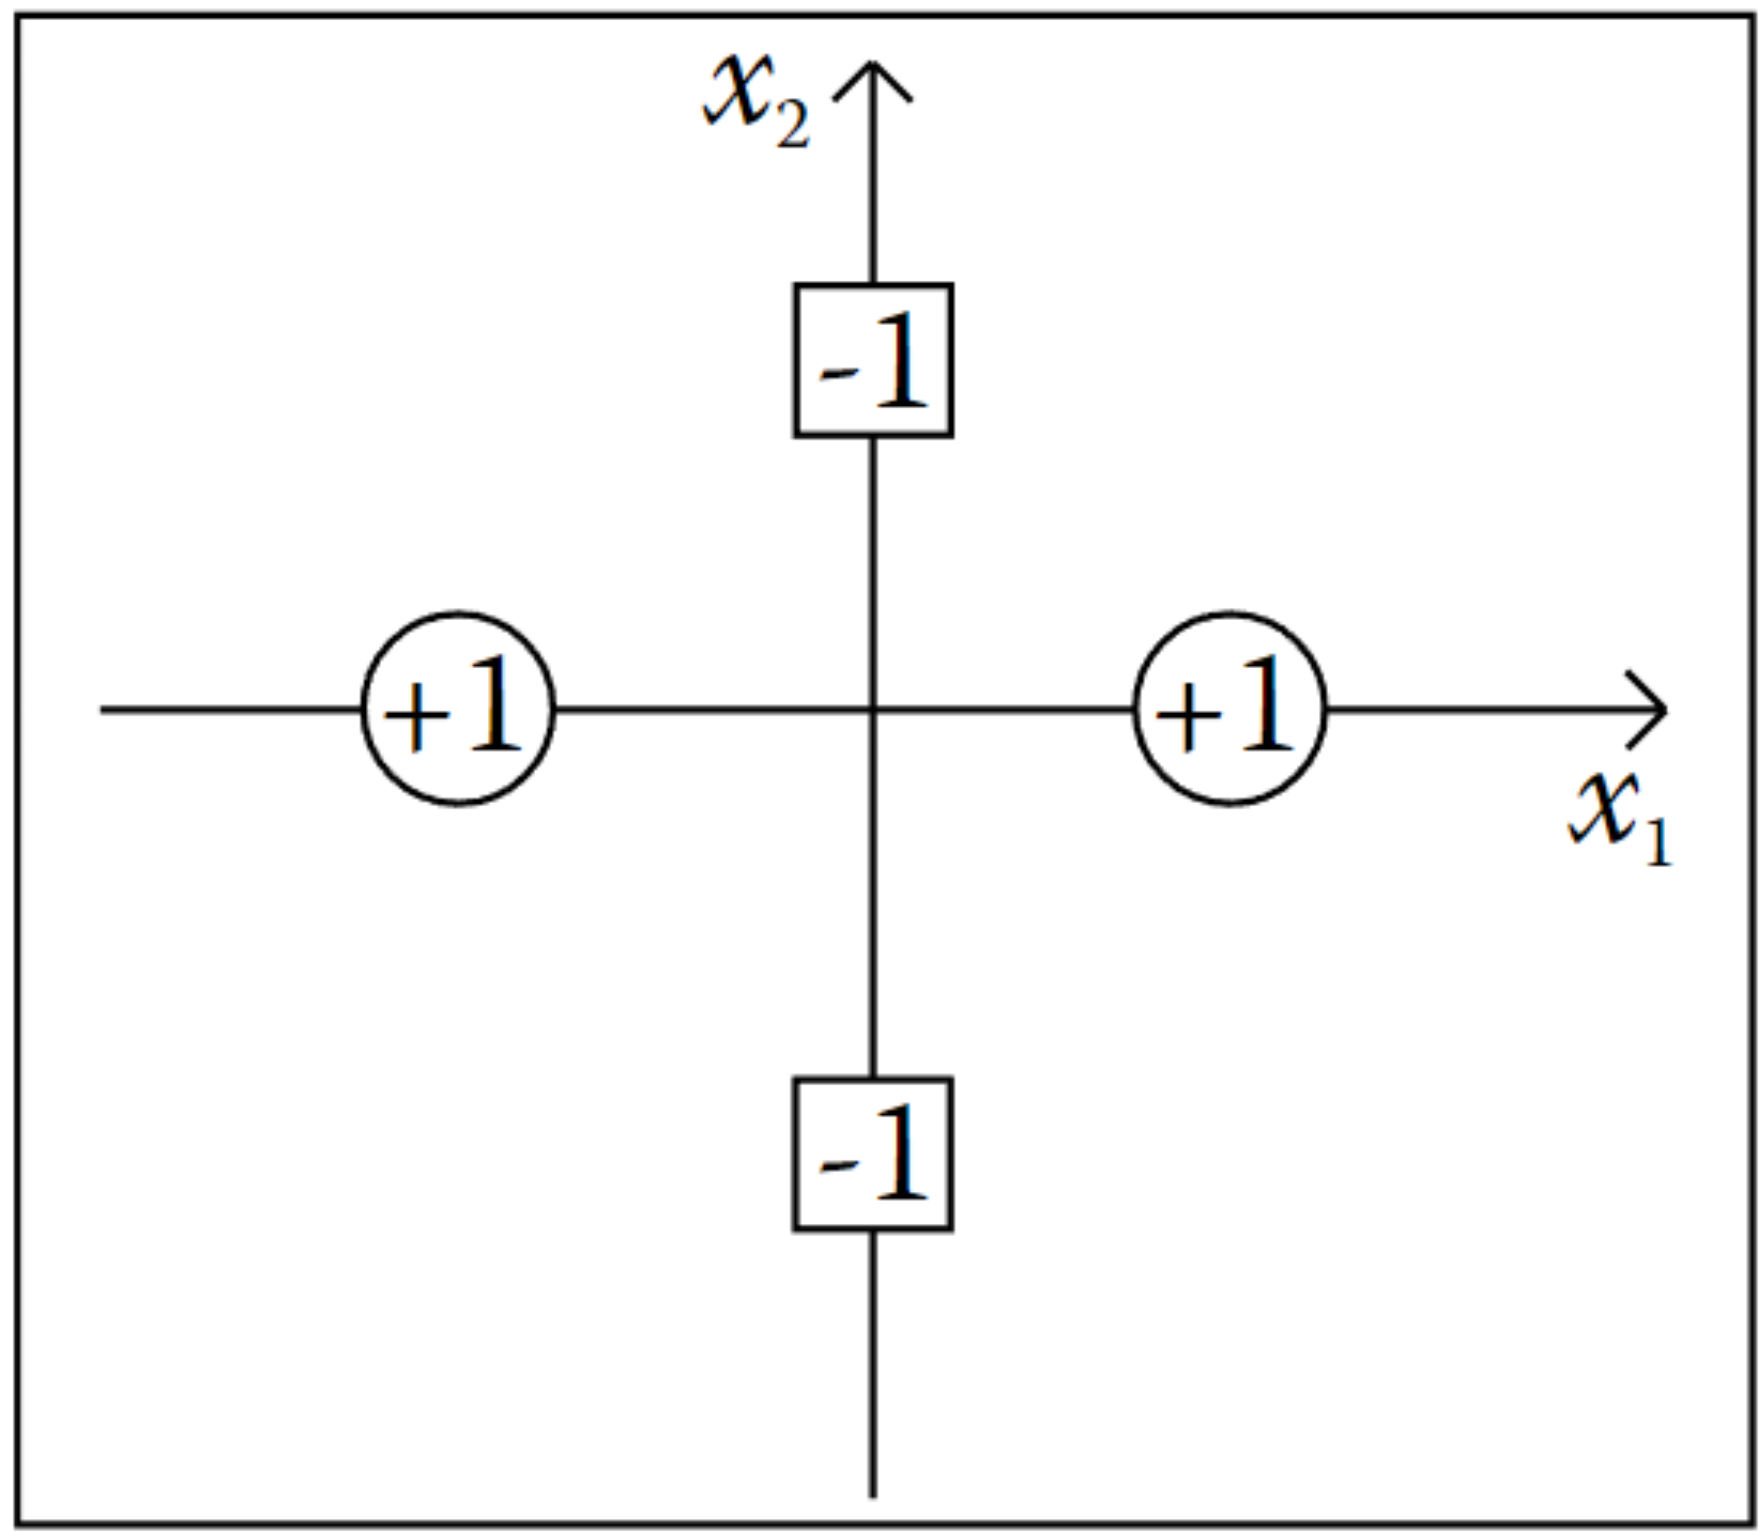
\includegraphics[width=0.5\textwidth]{figures/XOR-Problem.png}
    \caption[]{Visualisierung des XOR-Problems}
    \label{fig:XOR-Problem}
\end{figure*}
Wie aus Abbildung \ref*{fig:XOR-Problem} leicht zu erkennen ist, kann keine einfache Trennlinie gezogen werden, um
$+1$ und $-1$ voneinander zu trennen.\\
Nehmen wir nun an, dass durch den Lernalgorithmus nun acht Modelle als Funktionen vorliegen:
\begin{align*}
    h_1(x)=\left\{\begin{array}{r c}
                      +1, & \text{ wenn } (x_1 > -0.5) \\
                      -1, & \text{sonst}
                  \end{array}\right. &
    h_2(x)=\left\{\begin{array}{r c}
                      -1, & \text{ wenn } (x_1 > -0.5) \\
                      +1, & \text{sonst}
                  \end{array}\right. \\[10pt]
    h_3(x)=\left\{\begin{array}{r c}
                      +1, & \text{ wenn } (x_1 > +0.5) \\
                      -1, & \text{sonst}
                  \end{array}\right. &
    h_4(x)=\left\{\begin{array}{r c}
                      -1, & \text{ wenn } (x_1 > +0.5) \\
                      +1, & \text{sonst}
                  \end{array}\right. \\[10pt]
    h_5(x)=\left\{\begin{array}{r c}
                      +1, & \text{ wenn } (x_2 > -0.5) \\
                      -1, & \text{sonst}
                  \end{array}\right. &
    h_6(x)=\left\{\begin{array}{r c}
                      -1, & \text{ wenn } (x_2 > -0.5) \\
                      +1, & \text{sonst}
                  \end{array}\right. \\[10pt]
    h_7(x)=\left\{\begin{array}{r c}
                      +1, & \text{ wenn } (x_2 > +0.5) \\
                      -1, & \text{sonst}
                  \end{array}\right. &
    h_8(x)=\left\{\begin{array}{r c}
                      -1, & \text{ wenn } (x_2 > +0.5) \\
                      +1, & \text{sonst}
                  \end{array}\right. \\[10pt]
\end{align*}
\begin{enumerate}
    \item Der erste Schritt besteht darin, den Basis-Lernalgorithmus auf den ursprünglichen Daten aufzurufen.
          $h_2, h_3, h_5$ und $h_8$ haben alle eine Klassifikationsfehler von 0.25. Angenommen, $h_2$ wird als erster
          Basis-Lerner ausgewählt. Ein Datensatz $(x_1)$ wird falsch klassifiziert, daher beträgt der Fehler 0.25.
          Das Gewicht von $h_2$ beträgt ungefähr $\varepsilon_t\approx 0.55$. Abbildung \ref*{fig:XOR-Solution}(b) zeigt die Klassifikation und die Gewichtungen.
    \item Das Gewicht von $x_1$ wird erhöht und der Basis-Lernalgorithmus erneut aufgerufen. Diesmal haben $h_3, h_5$ und $h_8$
          gleiche Fehler. Angenommen, $h_3$ wird ausgewählt, dessen Gewicht 0.80 beträgt. Abbildung \ref*{fig:XOR-Solution}(c)
          zeigt die kombinierte Klassifikation von $h_2$ und $h_3$.
    \item Das Gewicht von $x_3$ wird erhöht. Diesmal haben nur $h_5$ und $h_8$ die niedrigsten Fehler. Angenommen, $h_5$ wird
          ausgewählt, dessen Gewicht 1.10 beträgt. Abbildung \ref*{fig:XOR-Solution}(d) zeigt die kombinierte Klassifikation
          von $h_2, h_3$ und $h_8$. Durch die Kombination der unvollkommenen linearen Klassifikatoren hat AdaBoost einen nichtlinearen Klassifikator mit
          null Fehler erzeugt.
\end{enumerate}
\begin{figure*}
    \centering
    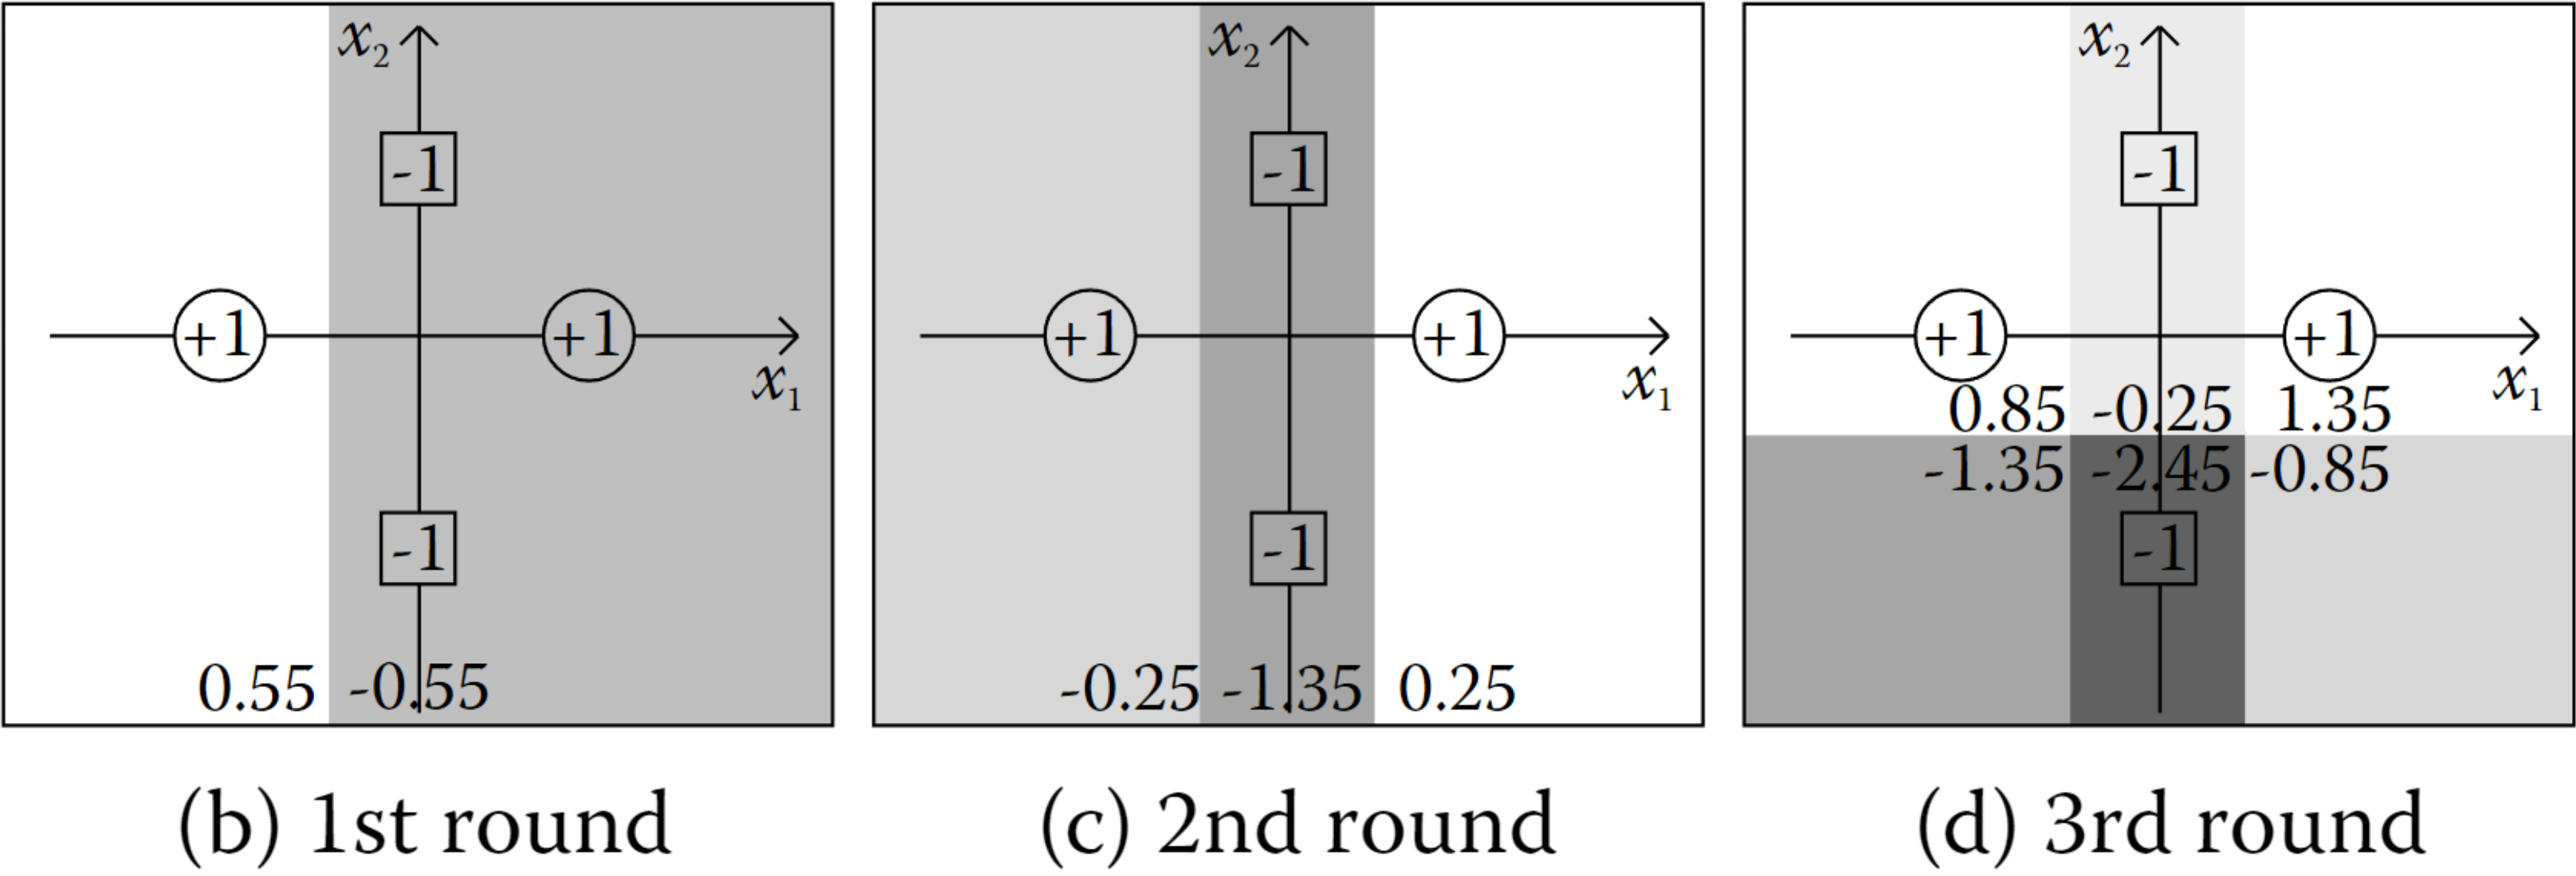
\includegraphics[width=0.7\textwidth]{figures/XOR_Solution.png}
    \caption[]{Visualisierung von AdaBoost auf dem XOR-Problem}
    \label{fig:XOR-Solution}
\end{figure*}
\section{Praktische Anwendung und Beispiele}
Vor allem wegen seiner Effizienz und Genauigkeit hat sich  in einer Vielzahl
von Anwendungen bewährt:
\begin{itemize}
    \item \textbf{Bilderkennung und Computervision:} Gesichtserkennung~\cite{viola2001rapid}
          \begin{figure*}
              \centering
              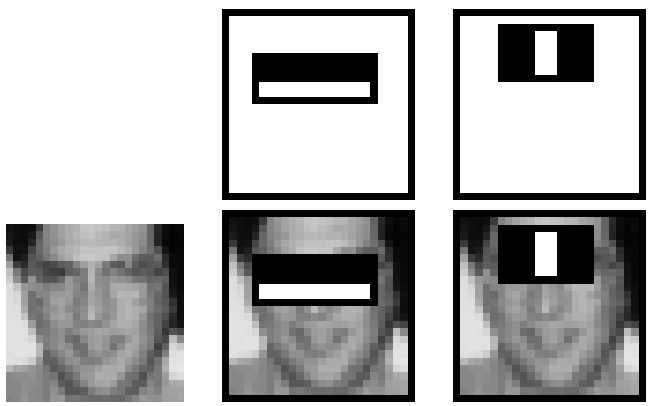
\includegraphics[width=.65\textwidth]{figures/CV_Example.png}
              \caption{Anwendung von AdaBoost bei Computer Vision:
                  Features messen Kontraste in bestimmten Gesichtsregionen\cite{viola2001rapid}}
          \end{figure*}
    \item \textbf{Textklassifikation und Natural Language Processing}: Erkennung von Spam-Mail~\cite{panwar2022detection}
          \begin{figure*}
              \centering
              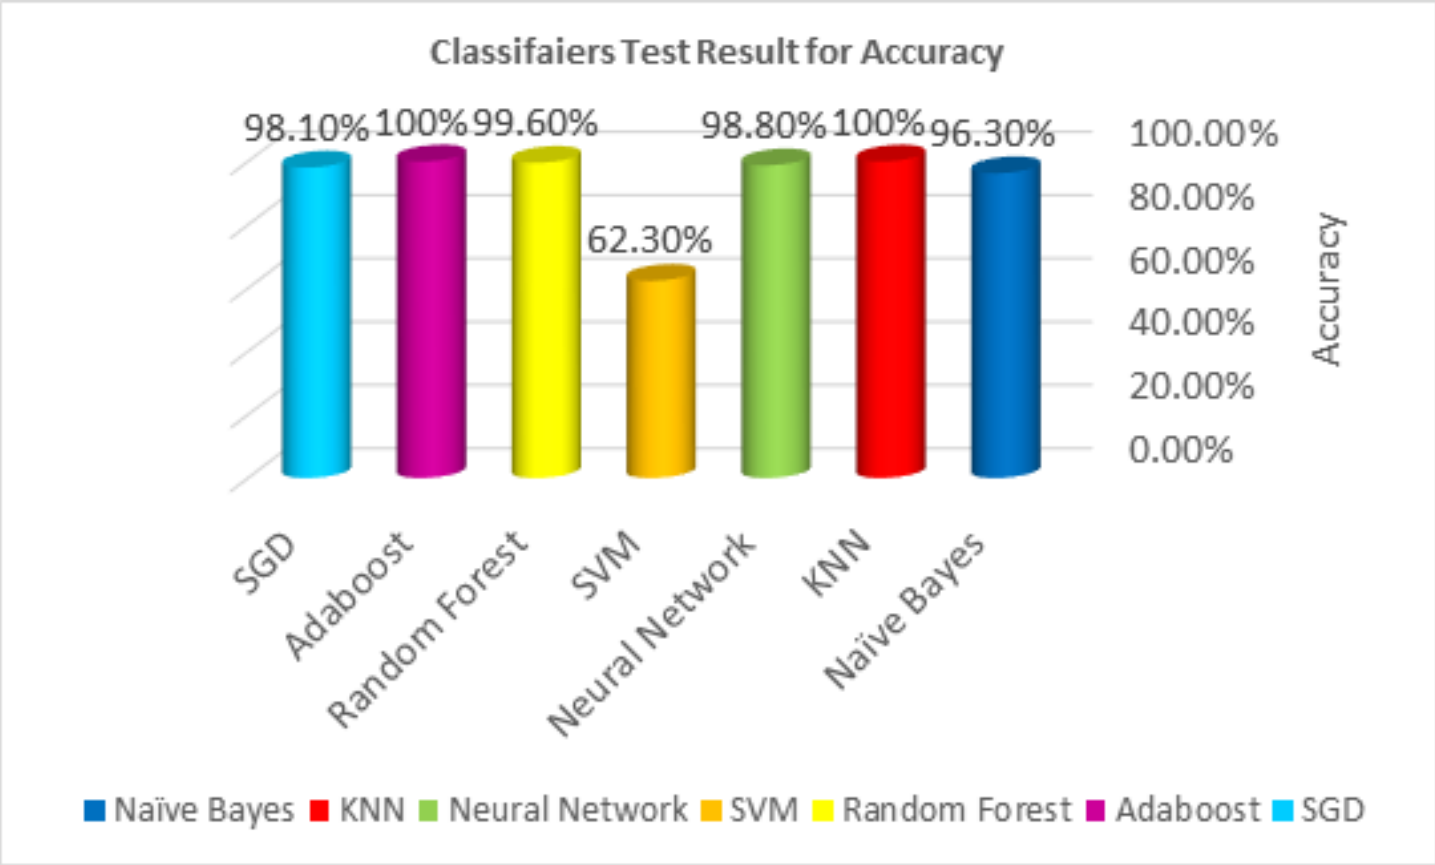
\includegraphics[width=.65\textwidth]{figures/spam.png}
              \caption{Erkennung von Spam-Mail durch AdaBoost im Vergleich zu anderen Verfahren\cite{panwar2022detection}}
          \end{figure*}
    \item \textbf{Medizinische Diagnostik:} Risiko/Erkennung von Krankheiten baserend auf Patientendaten~\cite{hatwell2020ada}
          \begin{figure*}
              \centering
              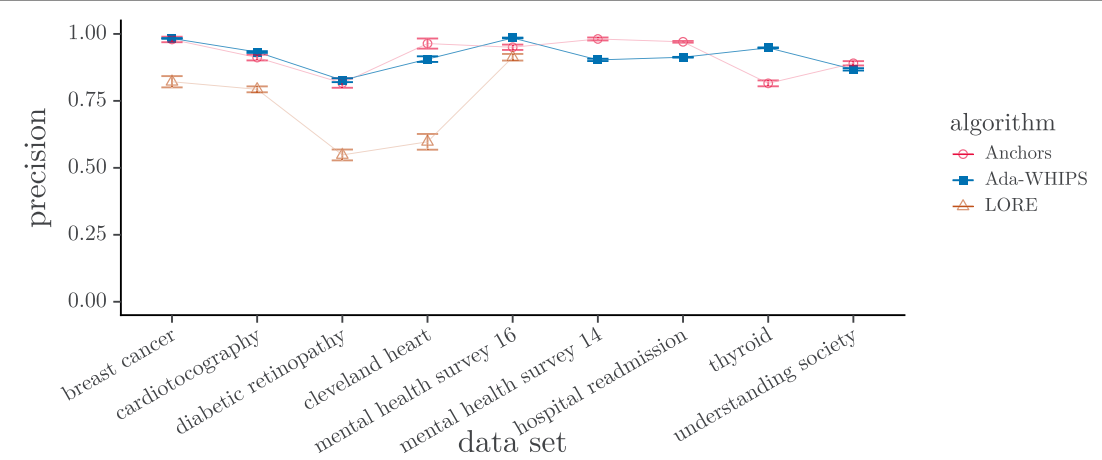
\includegraphics[width=.65\textwidth]{figures/ada-whips.png}
              \caption{Diagnostik mit AdaBoost im Vergleich \cite{hatwell2020ada}}
          \end{figure*}
    \item \textbf{Finanzwesen:} Vorhersage von Aktienkursbewegungen~\cite{zhang2016stock}
          \begin{figure*}
              \centering
              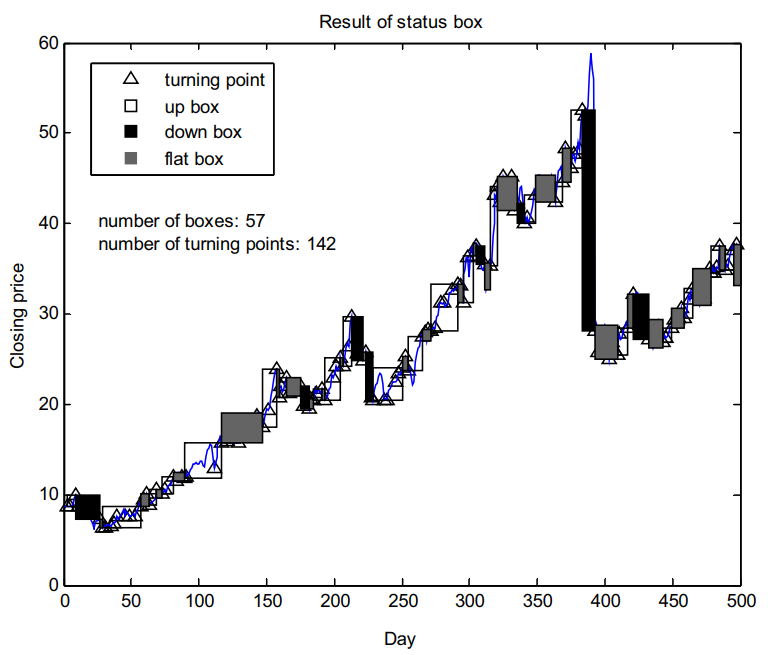
\includegraphics[width=.65\textwidth]{figures/stock.png}
              \caption{Vorhersage von Kursbewegungen mit AdaBoost. Boxen fassen Schlusspreise als Features zusammen. \cite{zhang2016stock}}
          \end{figure*}
\end{itemize}




\section{Vor- und Nachteile von AdaBoost}
AdaBoost ist einfach zu implementieren, vielseitig und benötigt oft keine Anpassung des Basislerners.
Er ist weniger anfällig für Overfitting und kann wichtige Features automatisch identifizieren.\\\\
Nachteile sind seine Empfindlichkeit gegenüber verrauschten Daten und Außreißern, der potenzielle Zeitaufwand bei großen
Datensätzen und seine Abhängigkeit vom Basislerner sowie seine Ausrichtung auf binäre Klassifikation.
\section{Erweiterungen und Variationen von AdaBoost}
AdaBoost, ursprünglich für binäre Klassifikation entwickelt,
wurde durch verschiedene Erweiterungen für diverse Problemstellungen adaptiert.

\begin{itemize}
    \item Variationen wie \glqq AdaBoost.M1\grqq~ und \glqq SAMME\grqq~ erweitern den Algorithmus für Multiklassen-Probleme.
    \item Kosten-sensitives AdaBoost passt Gewichtungen basierend auf Fehlerkosten an.
    \item Neben Entscheidungsstümpfen kann AdaBoost mit SVMs oder Neuronalen Netzen kombiniert werden.
    \item Robuste AdaBoost-Varianten minimieren die Auswirkung von Ausreißern.
    \item Online AdaBoost aktualisiert Modelle mit sequenziellen Daten ohne Neutrainierung.
    \item Einige Varianten integrieren Feature-Auswahl direkt, um Interpretierbarkeit und Trainingseffizienz zu steigern.
\end{itemize}
\newpage
% \section{Schlusswort}
% AdaBoost hat im Bereich des Ensemble-Lernens das maschinelle Lernen beeinflusst. Durch seine Einfachheit
und Leistungsfähigkeit ist er ein bis heute relevantes Werkzeug für Datenwissenschaftler.
\bibliographystyle{alpha}
\bibliography{seminar_top10.bib}

\end{document}